%%%%%%%%%%%%%%%%%%%%%%%%%%%%%%%%%%%%%%%%%%%%%%%%%%%%%%%%%%%%%%%%%%%%%%%%%%%%%%%%
%2345678901234567890123456789012345678901234567890123456789012345678901234567890
%        1         2         3         4         5         6         7         8
% THESIS CHAPTER

\chapter{Usage Scenarios}

This section discusses how the measure based approach implemented in The Vistorian could be used on three different networks. Brief summaries of the networks are provided.


\section{Scenario 1 [Marie Boucher]}
The Marie Boucher network \cite{dufournaud2017analyse}...
Summarise Marie Boucher background - I don't have this yet]

\begin{figure}[h!]
  \begin{center}
  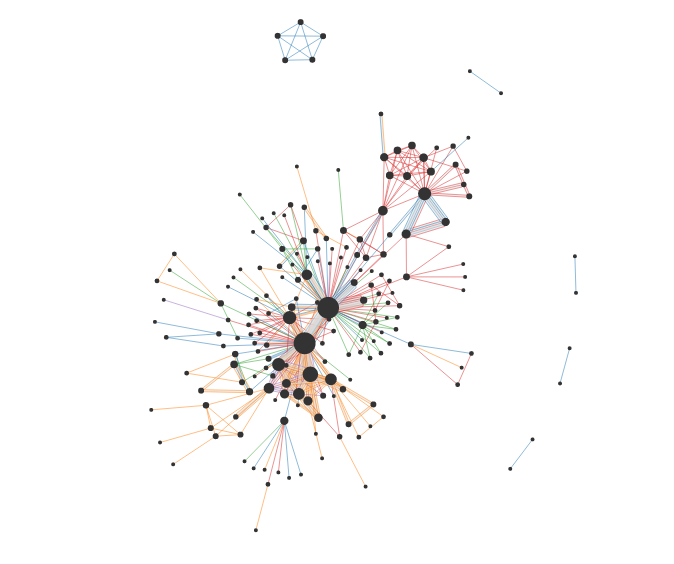
\includegraphics[trim={0 0 0 0}, width=140mm]{./Figures/marieBoucherFull.png}
  \caption{Marie Boucher network, full time period}
  \label{fig:marieBoucherFull}
  \end{center}
\end{figure}

-Only really one large component

-Some very central nodes

-Five satellite components

\begin{figure}[h!]
  \begin{center}
  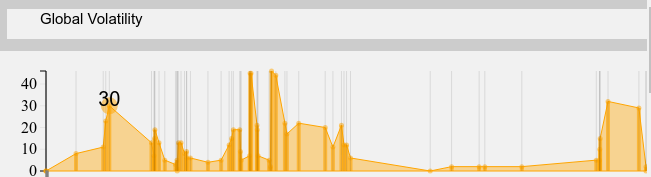
\includegraphics[trim={0 0 0 0}, width=140mm]{./Figures/marieBoucherGlobalVolatility.png}
  \caption{Marie Boucher Global Volatility}
  \label{fig:marieBoucherGlobalVolatility}
  \end{center}
\end{figure}

I'll begin by looking only at the global measures, starting with global volatility, Figure \ref{fig:marieBoucherGlobalVolatility}, we can see the network is initially erratic, then goes through very few changes for a sizeable portion of time, then has a burst of activity towards the end of the full period. 

\begin{figure}[h!]
  \begin{center}
  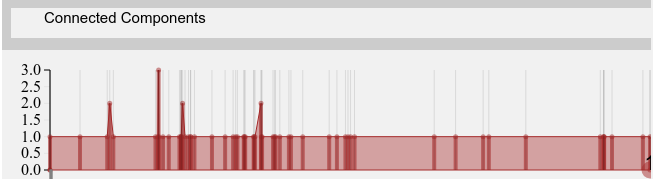
\includegraphics[trim={0 0 0 0}, width=140mm]{./Figures/marieBoucherConnectedComponents.png}
  \caption{Marie Boucher Connected Components}
  \label{fig:marieBoucherConnectedComponents}
  \end{center}
\end{figure}

Looking next at the number of connected components, Figure \ref{fig:marieBoucherConnectedComponents}, we find that for the majority of time frames there is only one connected component - there are three frames with two connected components and one frame with three connected components. Manually stepping through the graph we can also see that these components tend to be connected to one of two highly central nodes.

\begin{figure}[h!]
  \begin{center}
  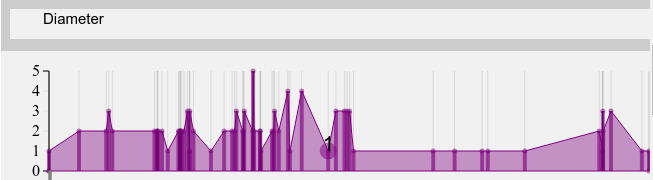
\includegraphics[trim={0 0 0 0}, width=140mm]{./Figures/marieBoucherDiameter.png}
  \caption{Marie Boucher Diameter}
  \label{fig:marieBoucherDiameter}
  \end{center}
\end{figure}

Looking next at Diameter, Figure \ref{fig:marieBoucherDiameter}, we see the same pattern we noticed in Global Volatility, erratic at first, a flat period of low activity then a jump at the end. There is a lot of variation in the values which could indicate that the network is quite different at each time frame. This is further enforced by density since it is similarly high in variation.

\begin{figure}[h!]
  \begin{center}
  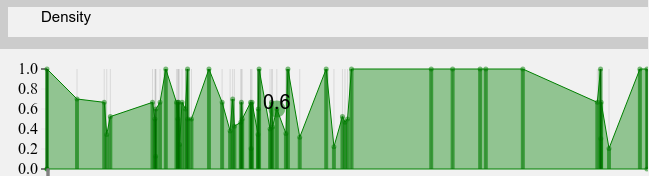
\includegraphics[trim={0 0 0 0}, width=140mm]{./Figures/marieBoucherDensity.png}
  \caption{Marie Boucher Density}
  \label{fig:marieBoucherDensity}
  \end{center}
\end{figure}

Density, \ref{fig:marieBoucherDensity}, follows the same pattern. Interestingly the density during the flat period is 100\%. Investigating this with the timeline slider we see that this is because there are only ever two nodes connected at a time during this period. 

\begin{figure}[h!]
  \begin{center}
  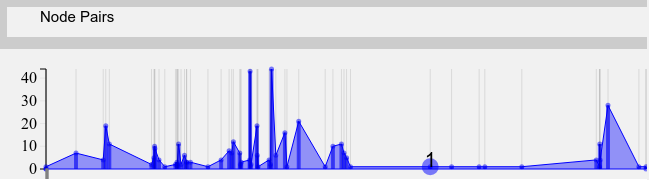
\includegraphics[trim={0 0 0 0}, width=140mm]{./Figures/marieBoucherNodePairs.png}
  \caption{Marie Boucher Node Pairs}
  \label{fig:marieBoucherNodePairs}
  \end{center}
\end{figure}

\begin{figure}[h!]
  \begin{center}
  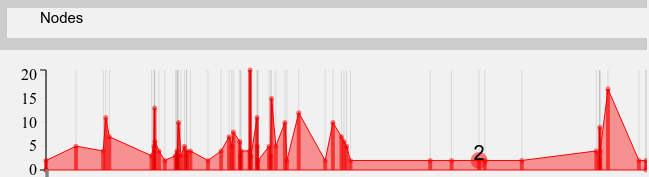
\includegraphics[trim={0 0 0 0}, width=140mm]{./Figures/marieBoucherNodes.png}
  \caption{Marie Boucher Nodes}
  \label{fig:marieBoucherNodes}
  \end{center}
\end{figure}

We could equally have confirmed this by looking at the number of node pairs, Figure \ref{fig:marieBoucherNodePairs}, and number of nodes, Figure \ref{fig:marieBoucherNodes}. The number of nodes is always 2 and number of nodepairs is always 1 during this flat period. The number of node pairs is very tightly correlated to the number of nodes here, the peaks could be worth further investigation as they are clearly periods of high activity relative to other frames.

\begin{figure}[h!]
  \begin{center}
  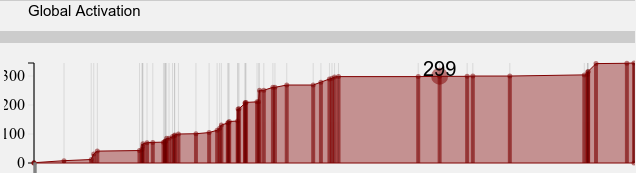
\includegraphics[trim={0 0 0 0}, width=140mm]{./Figures/marieBoucherGlobalActivation.png}
  \caption{Marie Boucher Global Activation}
  \label{fig:marieBoucherGlobalActivation}
  \end{center}
\end{figure}
Global activation, Figure \ref{fig:marieBoucherGlobalActivation} increases reasonably linearly for the first period. Notably during the flatter period it does increase slightly at each step confirming that the pairs we investigated in the density section are all different. 

\begin{figure}[h!]
  \begin{center}
  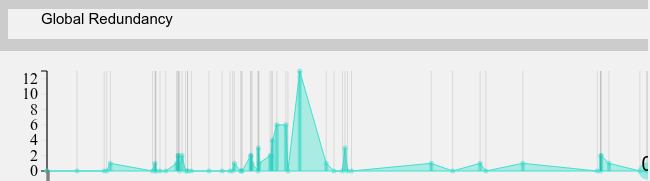
\includegraphics[trim={0 0 0 0}, width=140mm]{./Figures/marieBoucherGlobalRedundancy.png}
  \caption{Marie Boucher Global Redundancy}
  \label{fig:marieBoucherGlobalRedundancy}
  \end{center}
\end{figure}
Global redundancy, Figure \ref{fig:marieBoucherGlobalRedundancy}, is mostly fairly low, however there is one large peak which indicates further investigation could be useful as to why only that frame had many previously seen nodepairs, particularly as that specific frame wasn't identified as interesting by any of the other measures. The burst of activity at the end we noticed earlier isn't as obvious in this graph, indicating that most of the connections made in that period are new.
    
Looking more generally at the graphs, the spacing of the vertical lines also indicates three separate periods. We can also spot some periods and frames where many graphs have notable peaks or troughs that could spark further investigation.
    
\begin{center}
\begin{tabular}{cc}
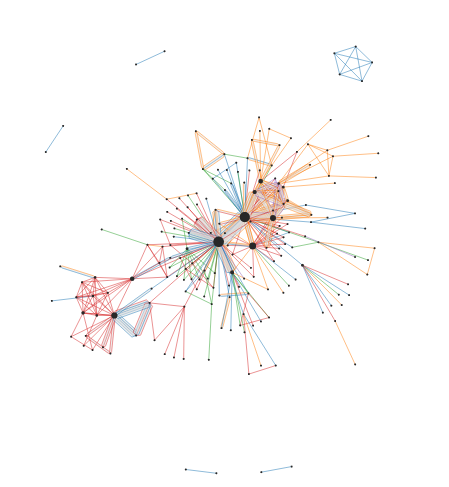
\includegraphics[trim={0 0 0 0}, width=140mm]{./Figures/marieBoucherLocalVolatilityFull.png}
\end{tabular}
\captionof{figure}{Marie Boucher - Local Volatility for the full time period}
\label{fig:marieBoucherLocalVolatilityFull}
\end{center}   
Next, the local measures can be investigated. Applying local volatility to the whole graph, Figure \ref{fig:marieBoucherLocalVolatilityFull}, we see that the two highly central nodes have high volatilities. This is because they make many fresh connections. Other fairly central nodes can be seen to have noticeably high volatilites. Standout nodes of interest here are more obvious than when the centrality measure is applied, as seen in Figure \ref{fig:marieBoucherLocalCentralityFull}.
\begin{center}
\begin{tabular}{cc}
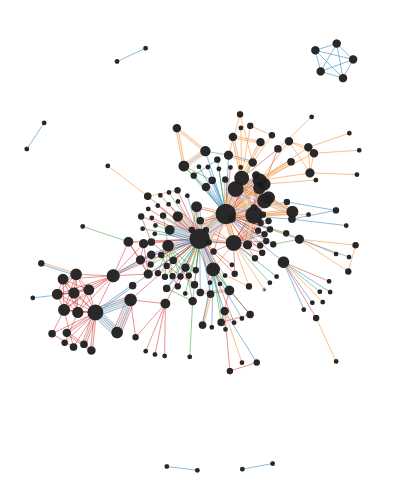
\includegraphics[trim={0 0 0 0}, width=85mm]{./Figures/marieBoucherLocalCentralityFull.png}
\end{tabular}
\captionof{figure}{Marie Boucher - Local Degree Centrality for the full period}
\label{fig:marieBoucherLocalCentralityFull}
\end{center}   


\begin{center}
\begin{tabular}{cc}
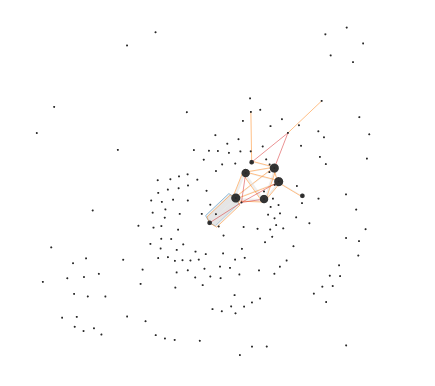
\includegraphics[trim={0 0 0 0}, width=85mm]{./Figures/marieBoucherLocalRedundancyPeriod1.png}
\end{tabular}
\captionof{figure}{Marie Boucher - Local Redundancy for a short period}
\label{fig:marieBoucherLocalRedundancyPeriod1}
\end{center}   
Applying local redundancy to the network, Figure \ref{fig:marieBoucherLocalRedundancyPeriod1}, and stepping through it, there are few nodes that particularly stand out as having high redundancy, as expected the central nodes tend to have higher values than the outer nodes but some of the tightly linked nodes have notable redundancies, showing that they are connected a few separate times in the full period.

\begin{center}
\begin{tabular}{cc}
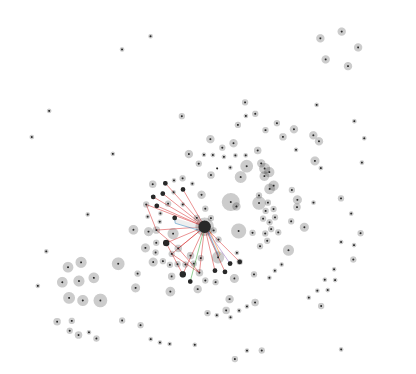
\includegraphics[trim={0 0 0 0}, width=140mm]{./Figures/marieBoucherLocalActivationPeriod1.png}
\end{tabular}
\captionof{figure}{Marie Boucher - Local Activation for a short period}
\label{fig:marieBoucherLocalActivationPeriod1}
\end{center} 
Switching to activation, Figure \ref{fig:marieBoucherLocalActivationPeriod1}, and we can see many nodes score quite high as we step through the network. The central nodes in particular but also some of the outer nodes.

\section{Scenario 2 Turin Network}

[Reference and Summary]

The Turin network is much more seperated than Marie Boucher and much more cluster/component based. This makes it an excellent network to analyse alongside Marie Boucher.

\begin{center}
\begin{tabular}{cc}
\label{edgeTypes}
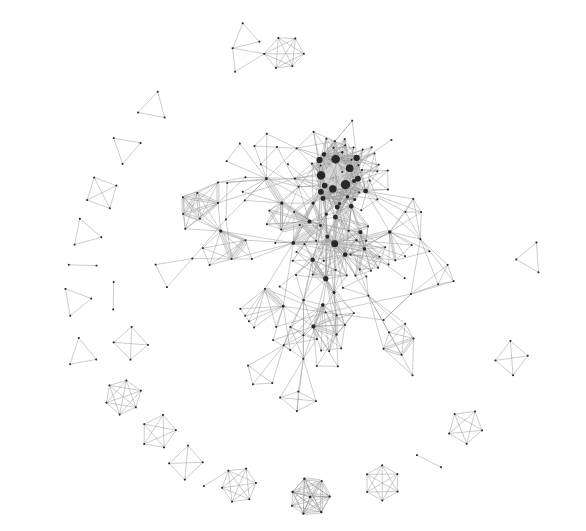
\includegraphics[trim={0 0 0 0}, width=140mm]{./Figures/TurinLocalVolatilityFull.png}
\end{tabular}
\captionof{figure}{The Turin Network, Local Volatility Measure Enabled}
\label{fig:TurinLocalVolatilityFull}
\end{center}

We begin again by looking at the global measures. Global volatility, Figure \ref{fig:TurinGlobalVolatility}, has around five periodic large jumps.

\begin{figure}[h!]
  \begin{center}
  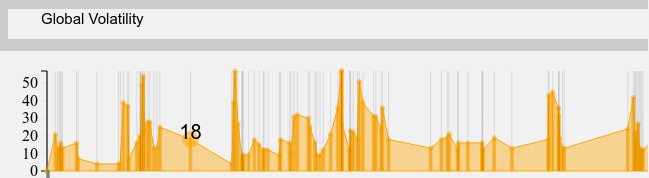
\includegraphics[trim={0 0 0 0}, width=140mm]{./Figures/TurinGlobalVolatility.png}
  \caption{Turin Global Volatility}
  \label{fig:TurinGlobalVolatility}
  \end{center}
\end{figure}

In between each of these jumps is reasonably high volatility, so together these indicate that there are occasional very large changes in the network and that in general the network is quite volatile and never really static for a period of time.
    
\begin{center}
\end{center}  

\begin{figure}[h!]
  \begin{center}
  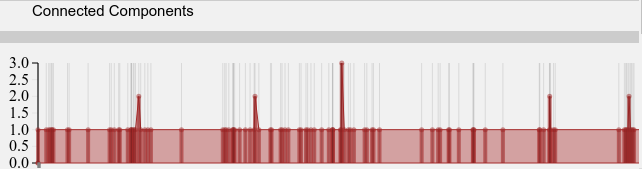
\includegraphics[trim={0 0 0 0}, width=140mm]{./Figures/TurinConnectedComponents.png}
  \caption{Turin Connected Components}
  \label{fig:TurinConnectedComponents}
  \end{center}
\end{figure}
Looking next at the number of connected components, Figure \ref{fig:TurinConnectedComponents} ,if we observe the network itself and step through it then it is readily apparent that it is made of many small connected components which tend to become active for short periods. Interestingly, what this graph shows - combined with this observation about the network, is that for the majority of the time there is only one active connected component, with only four time frames occurring with two active and one time frame occurring with three active.

\begin{figure}[h!]
  \begin{center}
  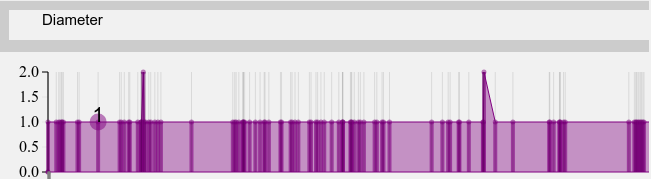
\includegraphics[trim={0 0 0 0}, width=140mm]{./Figures/TurinDiameter.png}
  \caption{Turin Diameter}
  \label{fig:TurinDiameter}
  \end{center}
\end{figure}
Diameter, Figure \ref{fig:TurinDiameter}, is equally interesting, there are only two time frames where the diameter is over one, and in both cases that value is two. Combined with what we know about connected components we can see that all of these components are highly connected since the vast majority only have a diameter of one, which is the smallest possible diameter for any network.
    
\begin{figure}[h!]
  \begin{center}
  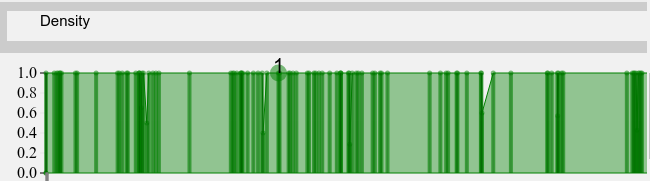
\includegraphics[trim={0 0 0 0}, width=140mm]{./Figures/TurinDensity.png}
  \caption{Turin Density}
  \label{fig:TurinDensity}
  \end{center}
\end{figure}
Adding density, Figure \ref{fig:TurinDensity}, further consolidates these findings as we can see that for the majority of time frames the components have a density of $1.0$. Combining this with what we've already discovered we now know that in most time frames we have a single connected component with every node in that component connected to every other node in that component. Two of the dips also align with the spikes in diameter.

\begin{figure}[h!]
  \begin{center}
  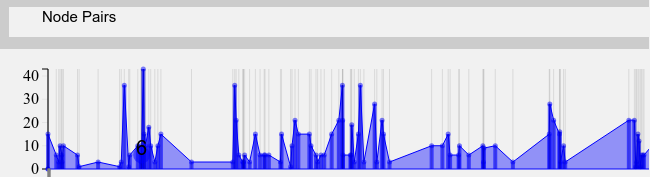
\includegraphics[trim={0 0 0 0}, width=140mm]{./Figures/TurinNodePairs.png}
  \caption{Turin Nodepairs}
  \label{fig:TurinNodePairs}
  \end{center}
\end{figure}

\begin{figure}[h!]
  \begin{center}
  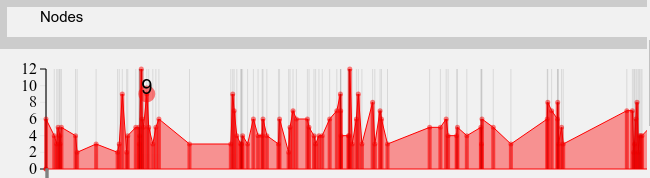
\includegraphics[trim={0 0 0 0}, width=140mm]{./Figures/TurinNodes.png}
  \caption{Turin Nodes}
  \label{fig:TurinNodes}
  \end{center}
\end{figure}
Due to the density and what we've observed previously, the number of nodepairs, Figure \ref{fig:TurinNodePairs}, and nodes, Figure \ref{fig:TurinNodes}, are naturally very tightly correlated. Comparing with the density graph we can see that the few blips in perfect correlation all match the fluctuations in density. Since we know this network tends to have one active fully connected component active in each time frame, we can now gain a sense of the sizes of each of these components. Comparing again with the connected components graph we can see that these large jumps tend to be linked with time frames where there is more than one connected component. Some of the blips in diameter and density also align with time frames with more than one connected component. The time frames these blips occur in could therefore be worth extra investigation.
    
\begin{figure}[h!]
  \begin{center}
  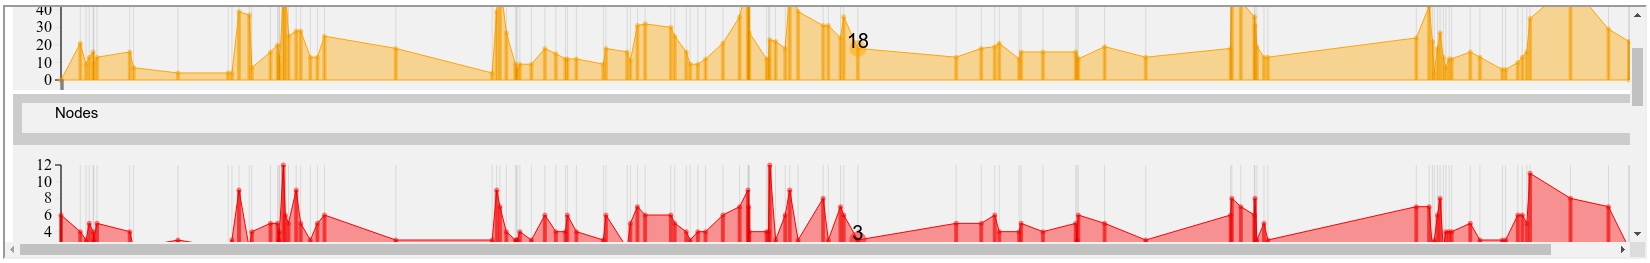
\includegraphics[trim={0 0 0 0}, width=140mm]{./Figures/TurinGlobalVolatilityAndNodes.png}
  \caption{Turin Global Volatility and Nodes comparison}
  \label{fig:TurinGlobalVolatilityAndNodes}
  \end{center}
\end{figure}

Comparing number of nodes with Global Volatility, Figure \ref{fig:TurinGlobalVolatilityAndNodes}, by dragging the number of nodes graph up such that it is directly below the global volatility graph they can now be easily compared. We can see that the steps of very high volatility identified earlier are explained by the large new connected components appearing during those time frames.
   
\begin{figure}[h!]
  \begin{center}
  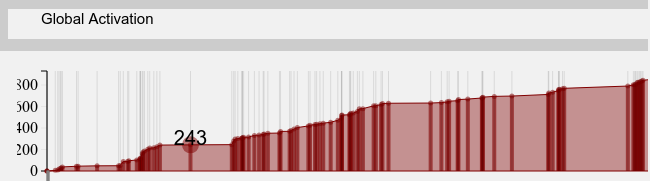
\includegraphics[trim={0 0 0 0}, width=140mm]{./Figures/TurinGlobalActivation.png}
  \caption{Turin Global Activation}
  \label{fig:TurinGlobalActivation}
  \end{center}
\end{figure}

Continuing down to Global Activation, Figure \ref{fig:TurinGlobalActivation}, we can see that new nodepairs are added at a fairly constant pace. Looking next at Global Redundancy, the peaks indicate that many of the nodepairs have been active before, we can use this alongside the network itself to easily find the components that appear more than once.

\begin{figure}[h!]
  \begin{center}
  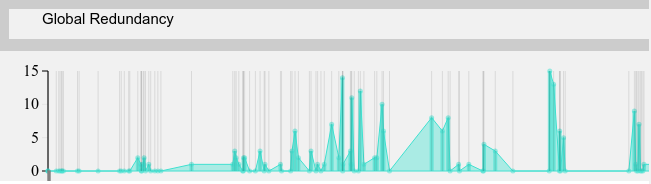
\includegraphics[trim={0 0 0 0}, width=140mm]{./Figures/TurinGlobalRedundancy.png}
  \caption{Turin Global Redundancy}
  \label{fig:TurinGlobalRedundancy}
  \end{center}
\end{figure}
Finally with Global Redundancy, Figure \ref{fig:TurinGlobalRedundancy}, the values appear highly erratic. This measure would be useful to see at which periods past business groups are reconnected. Dragging it to compare it with Global Volatility and Nodepairs we can see some correlation.


Looking more generally at all graphs we can gain some more insight. Looking at the spread of time frames by observing the vertical bars, we can identify periods of no change and periods of considerable change. 
    
\begin{center}
\end{center}

\begin{center}
\begin{tabular}{cc}
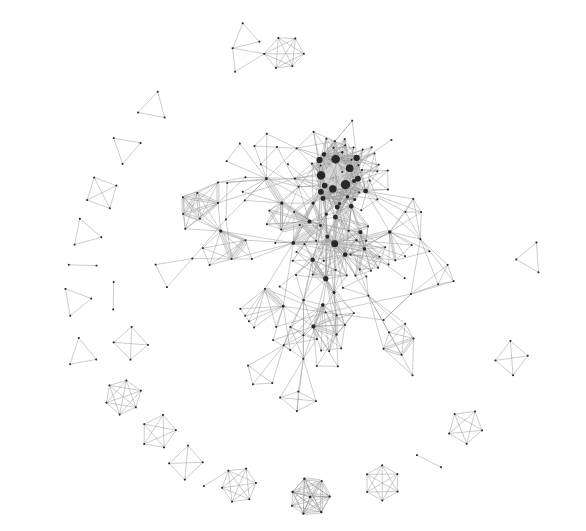
\includegraphics[trim={0 0 0 0}, width=140mm]{./Figures/TurinLocalVolatilityFull.png}
\end{tabular}
\captionof{figure}{Turin Local Volatility - Full time period}
\label{fig:TurinLocalVolatilityFull}
\end{center}
Next, we can experiment with the local measures. First with volatility, stepping through the network with a minimal window we see that the connected components tend to all have low similar volatilities with no standout nodes. Observing the full network over the whole time period we see that there is a large cluster containing several highly volatile nodes, Figure \ref{fig:TurinLocalVolatilityFull}. Stepping through the graph we see that this is because many of the connected components overlap in some way within this cluster of nodes. These nodes are therefore very worthy of further investigation as they are highly active and with many different nodes rather than a fixed number.


\begin{center}
\begin{tabular}{cc}
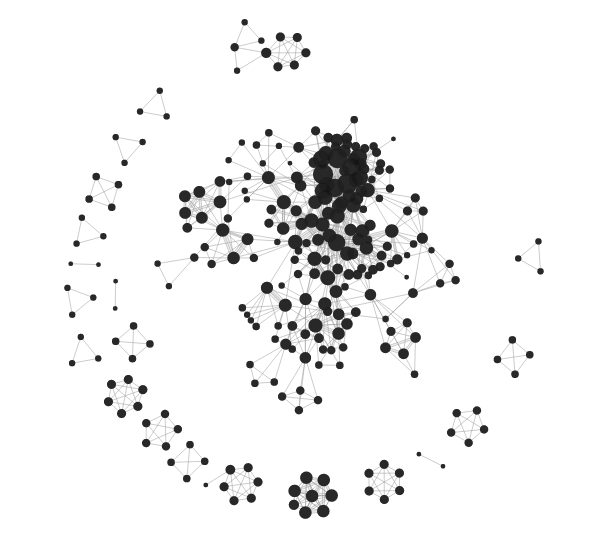
\includegraphics[trim={0 0 0 0}, width=140mm]{./Figures/TurinLocalCentralityFull.png}
\end{tabular}
\captionof{figure}{Turin Centrality - Full time period}
\label{fig:TurinLocalCentralityFull}
\end{center}

\begin{center}
\end{center}
Comparing these results from local volatility with the centrality measure - again applied to the whole graph, Figure \ref{fig:TurinLocalCentralityFull} - is interesting, because we can see that using local volatility makes the interesting nodes stand out much more. 
\begin{center}
\begin{tabular}{cc}
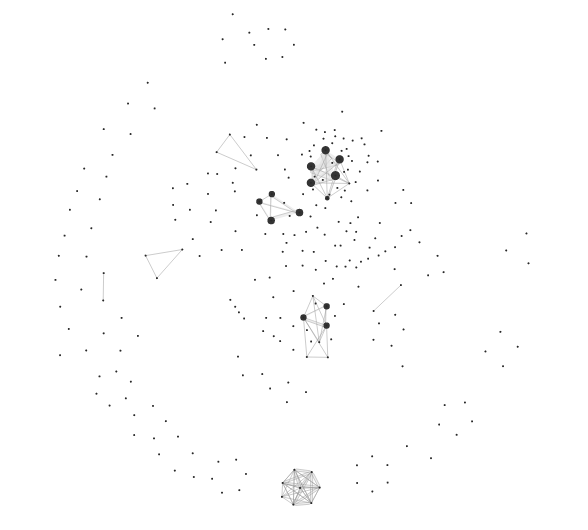
\includegraphics[trim={0 0 0 0}, width=140mm]{./Figures/TurinLocalRedundancy1.png}
\end{tabular}
\captionof{figure}{Turin Local Redundancy - short time period}
\label{fig:TurinLocalRedundancy1}
\end{center}
Switching to local redundancy and selecting a period towards the end of the network's timeline, Figure \ref{fig:TurinLocalRedundancy1}, we can easily spot the components that have been active at some point before that period as they have a redundancy $> 0$. This further complements our findings from the global redundancy measure.

\begin{center}
\begin{tabular}{cc}
\label{edgeTypes}
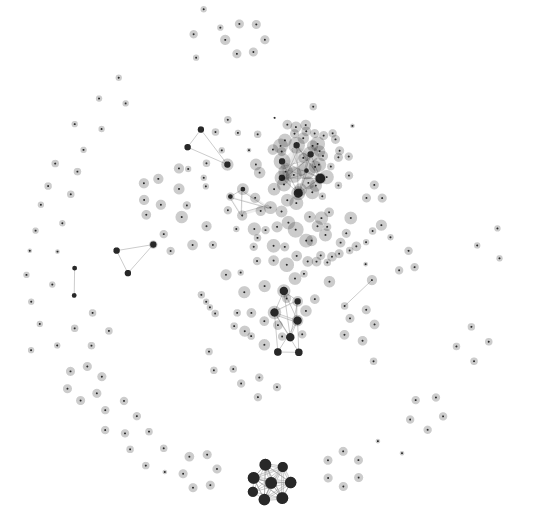
\includegraphics[trim={0 0 0 0}, width=140mm]{./Figures/TurinLocalActivation.png}
\end{tabular}
\captionof{figure}{Turin Local Activation - same short time period}
\label{fig:TurinLocalActivation}
\end{center}
Switching directly to local activation from here, Figure \ref{fig:TurinLocalActivation}, and looking again at the components identified as having higher redundancy we can see how high the activation in the selected time period is relative to the total network activity by comparing with the grey outer circles. Since they aren't considerably larger for any node in these components we could infer that this component is likely only fully active one or two times before this period.

\section{Scenario 3 - Marguerite} 

\begin{multicols}{2}
\begin{center}
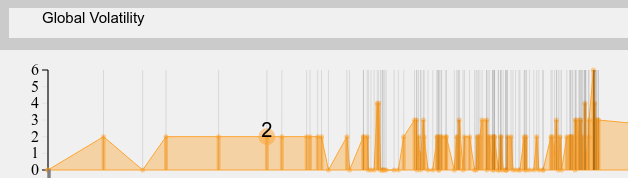
\includegraphics[trim={0 0 0 0}, width=60mm]{./Figures/margueriteGlobalVolatility.png}
\end{center}
\begin{center}
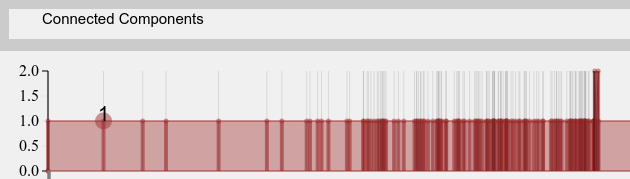
\includegraphics[trim={0 0 0 0}, width=60mm]{./Figures/margueriteConnectedComponents.png}
\end{center}
\begin{center}
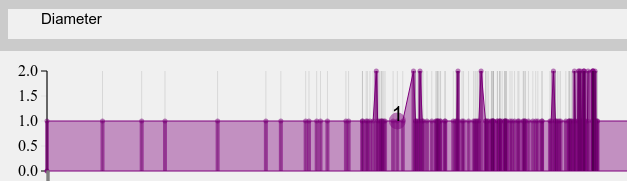
\includegraphics[trim={0 0 0 0}, width=60mm]{./Figures/margueriteDiameter.png}
\end{center}
\begin{center}
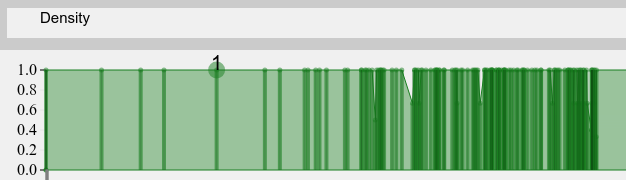
\includegraphics[trim={0 0 0 0}, width=60mm]{./Figures/margueriteDensity.png}
\end{center}
\begin{center}
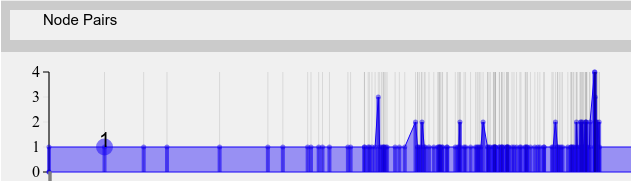
\includegraphics[trim={0 0 0 0}, width=60mm]{./Figures/margueriteNodePairs.png}
\end{center}
\begin{center}
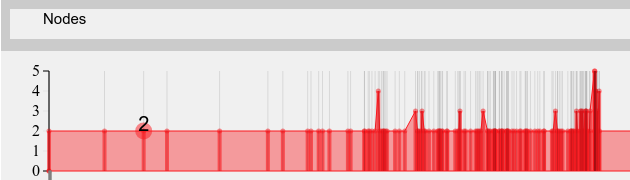
\includegraphics[trim={0 0 0 0}, width=60mm]{./Figures/margueriteNodes.png}
\end{center}
\begin{center}
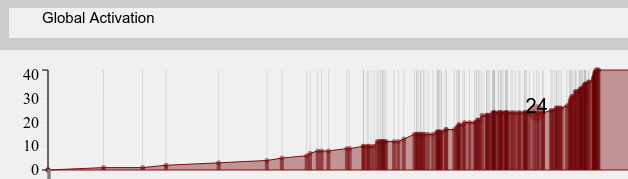
\includegraphics[trim={0 0 0 0}, width=60mm]{./Figures/margueriteGlobalActivation.png}
\end{center}
\begin{center}
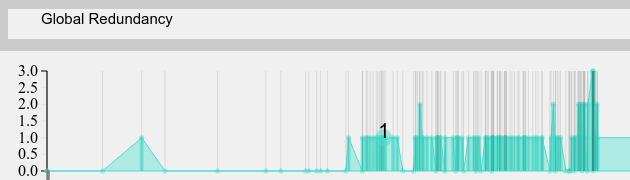
\includegraphics[trim={0 0 0 0}, width=60mm]{./Figures/margueriteGlobalRedundancy.png}
\end{center}
\captionof{figure}{All Global Measures for Marguerite Network}
\label{fig:margueriteAllGraphs}
\columnbreak
[Reference]
Finally, to assess the power of the measure based approach, we could try looking solely at the global measures of a new network to see how much information we can gleam, Figure \ref{fig:margueriteAllGraphs}. 

Looking generally at all graphs we can see there is fairly little activity in the first half and then a lot in the second. We can see that for most time frames there are only two nodes involved - explaining the density and diameter - and steadily increasing global activation implying that many new nodes are connected to. What's very interesting however is that global redundancy for the second half tends to be one. Tying this together and the picture we get is either of a network primarily composed of one node connecting to many new nodes in the second period or many pairs becoming active where one of the nodes in the pair has been active before. Looking more closely at the values of global activation which appear to increase by one during each time frame in this period and we can rule out the second option.
\end{multicols}

Looking at the actual network, Figure \ref{fig:margueriteNetwork}, these findings were accurate. 

\begin{figure}[h!]
  \begin{center}
  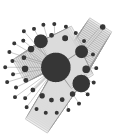
\includegraphics[trim={0 0 0 0}, width=40mm]{./Figures/margueriteNetwork.png}
  \caption{Marguerite Full Network}
  \label{fig:margueriteNetwork}
  \end{center}
\end{figure}
[Summary and reference for the Marguerite network.]
Of course, the measures are meant to be complementary to the network and not to replace it, but being able to extract this much information solely from them with relative ease indicates that they are a powerful tool.

\pagebreak
\section{Directly comparing Marie Boucher and Turin}
\begin{multicols}{2}
\begin{center}
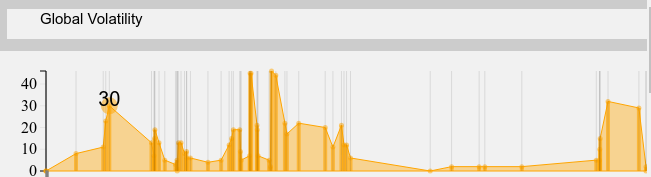
\includegraphics[trim={0 0 0 0}, width=60mm]{./Figures/marieBoucherGlobalVolatility.png}
\end{center}
\begin{center}
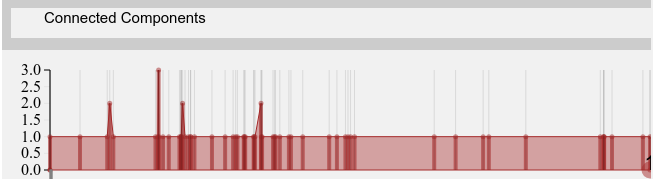
\includegraphics[trim={0 0 0 0}, width=60mm]{./Figures/marieBoucherConnectedComponents.png}
\end{center}
\begin{center}
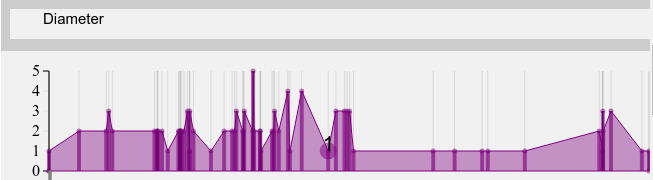
\includegraphics[trim={0 0 0 0}, width=60mm]{./Figures/marieBoucherDiameter.png}
\end{center}
\begin{center}
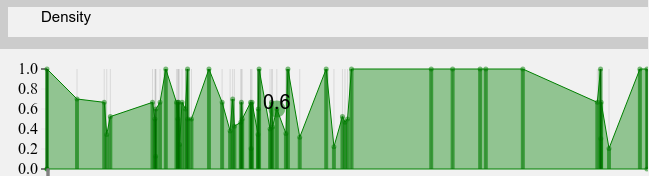
\includegraphics[trim={0 0 0 0}, width=60mm]{./Figures/marieBoucherDensity.png}
\end{center}
\begin{center}
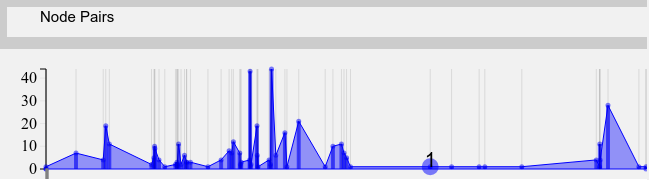
\includegraphics[trim={0 0 0 0}, width=60mm]{./Figures/marieBoucherNodePairs.png}
\end{center}
\begin{center}
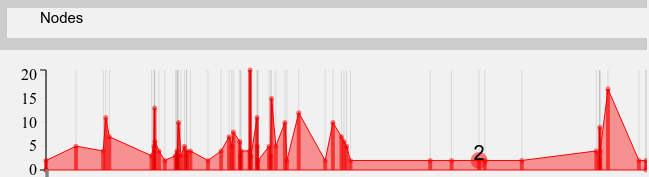
\includegraphics[trim={0 0 0 0}, width=60mm]{./Figures/marieBoucherNodes.png}
\end{center}
\begin{center}
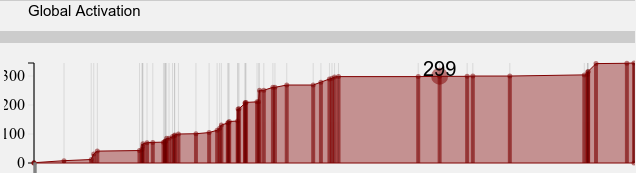
\includegraphics[trim={0 0 0 0}, width=60mm]{./Figures/marieBoucherGlobalActivation.png}
\end{center}
\begin{center}
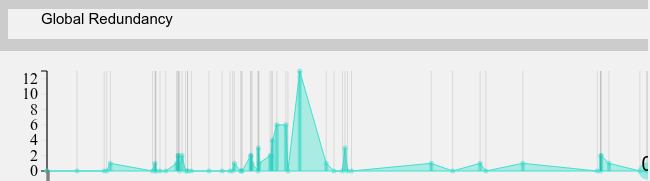
\includegraphics[trim={0 0 0 0}, width=60mm]{./Figures/marieBoucherGlobalRedundancy.png}
\end{center}
\captionof{figure}{Marie Boucher Network}
\label{fig:marieBoucherAllGraphs}
\columnbreak



\begin{center}
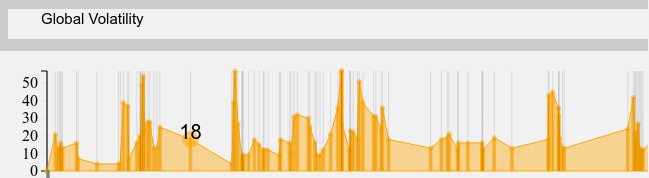
\includegraphics[trim={0 0 0 0}, width=60mm]{./Figures/TurinGlobalVolatility.png}
\end{center}
\begin{center}
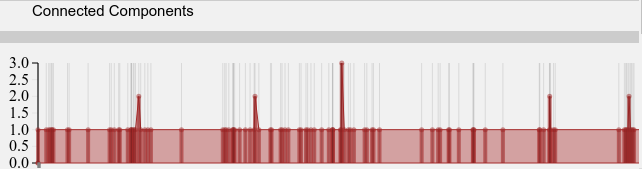
\includegraphics[trim={0 0 0 0}, width=60mm]{./Figures/TurinConnectedComponents.png}
\end{center}
\begin{center}
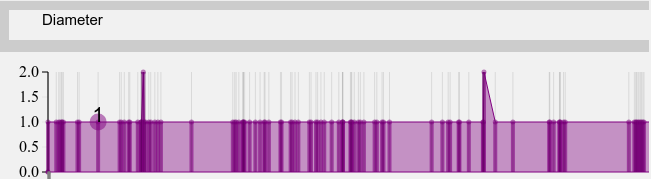
\includegraphics[trim={0 0 0 0}, width=60mm]{./Figures/TurinDiameter.png}
\end{center}
\begin{center}
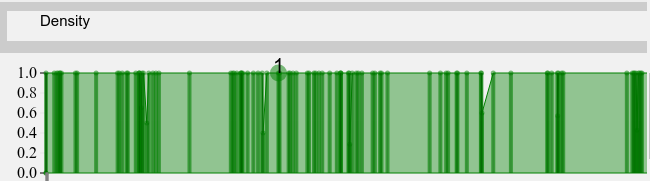
\includegraphics[trim={0 0 0 0}, width=60mm]{./Figures/TurinDensity.png}
\end{center}
\begin{center}
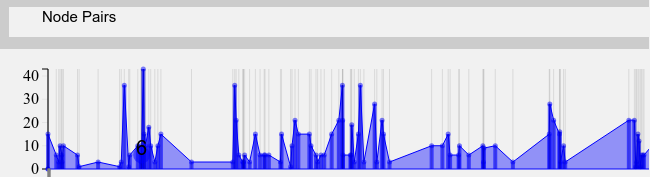
\includegraphics[trim={0 0 0 0}, width=60mm]{./Figures/TurinNodePairs.png}
\end{center}
\begin{center}
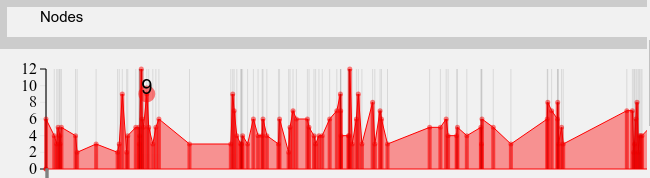
\includegraphics[trim={0 0 0 0}, width=60mm]{./Figures/TurinNodes.png}
\end{center}
\begin{center}
\includegraphics[trim={0 0 0 0}, width=60mm]{./Figures/TurinGlobalActivation.png}
\end{center}
\begin{center}
\includegraphics[trim={0 0 0 0}, width=60mm]{./Figures/TurinGlobalRedundancy.png}
\end{center}
\captionof{figure}{Turin Network}
\label{fig:turinAllGraphs}
\end{multicols}

Interestingly, When looking at the actual networks themselves, Figure \ref{fig:TurinLocalVolatilityFull} and Figure \ref{fig:marieBoucherFull}, despite the fact that they appear quite different, the global measure graphs, Figures \ref{fig:marieBoucherAllGraphs} and \ref{fig:turinAllGraphs}, seem quite similar at a glance. This is likely because whilst actually stepping through each time frame, the networks behave similarly in that there are usually only a few nodes involved and they tend to be in a single component. The difference, which can be seen in the diameter and density graphs, is that in the Marie Boucher network these components tend to be made up of one central node with the other active nodes mostly only connected to it, but in the Turin network, the nodes tend to be more interconnected.


\chapter{Discussion}

In this paper I have presented a measure based approach to dynamic network visualisation. Details of the measures and their implemented visualisation have been provided.

...

\section{Potential further work} 
Creating visualisations is a highly iterative and experimental process, so naturally many ideas have been produced for improvements that could be made to the system. This section details some of those potential improvements.
\newline

Automatically highlighting points of interest could be a useful feature, by looking at the "interestingness" of each timeframe. These points of interest would be timeframes where many of the global measures differ significantly from their average and could be considered outliers. The most significant, say, three of these timeframes could then be shown on the timeline. One possible way to achieve this that I considered would be using Tukey fences, which can be used to spot outliers. David C. Hoaglin in John W. Tukey and Data Analysis \cite{jwtada} states that Exploratory Data Analysis\cite{eda} uses "fences" to flag possible outliers. These are based on the "hinges," $H_L$ and $H_U$, which are approximate quartiles of the batch. He goes on to say that the basic idea is to calculate the H-spread, $d_H = H_U - H_L$, and lay off a multiple of it below $H_L$ and above $H_U$: 
\begin{equation}
 H_L-kd_H \, \, and \, \, H_U + kd_H.
\end{equation}
He continues to say that the limited preliminary edition (Tukey, 1970c) used k = 1.0 for the "side values" and k = 1.5 for the "three-halves values." By the first edition (Tukey, 1977a) the constants had changed a lot, to k = 1.5 for the "inner fences" and k = 3.0 for the "outer fences," with the labels "outside" and "far out," respectively, for data values beyond them.
Finally he states that the aim was not to have a formal rule for declaring an observation an outlier, but to call attention to such data for further investigation. The values of k have remained at 1.5 and 3.0, and the "inner fences" naturally see more use in practice. 
Since the goal is not to formally rule on outliers but rather to "call attention to such data for further investigation", this method could work well for calculating a sense of 'interestingness'.
\newline

Adding more measures is an obvious improvement - particularly local dynamic measures as they aren't found in other tools. An example could be a measure to add a sense of node 'promiscuity' - if volatility focuses on how the lifespans of node-pairs vary over time then 'promiscuity' would focus more on how often those edges tend to be with the same nodes. A node that had a few fairly rigid connections but also made a new connection every time step would have relatively low volatility but high promiscuity. A node that erratically gained and lost connections but only to a select few nodes would have high volatility but low promiscuity.
\newline

The grey node 'halos' shown in Figure \ref{fig:greyCircles} could be adjusted such that instead of being fixed to the full time period, the could be locked to the currently selected period with a button. This would allow a user to select one period, lock that selection so that the 'halos' are recalculated, then change their time period selection and compare the new node sizes with the "halo" sizes for a given local measure.
\newline

Adding the ability to move the databar into a separate window, which could then be dragged to a separate screen - creating more space for the node-link diagram and allowing more graphs in the databar to be visualised at once. 
\newline

Running a think-aloud study or similar user trial could be useful to discover more about how effective the current implementation is and provide insight into further improvements.
\newline

Another improvement mentioned during the feedback meeting (and briefly considered before) was enabling graphs to be exported as a png to allow for easy insertion into academic papers. This would encourage adoption and improve quality of life for end users.
\newline


\section{Evaluation of work completed} 
The meeting with network scientists validated the approach and the system works well in the described usage scenarios. I'm confident that a measure based approach works well as a dynamic network visualisation when used alongside a nodelink diagram. More specifically, most measures appear to be useful in their own right although there can be occasional overlap in the information they provide. The number of connected components measure could perhaps be replaced with a cluster based measure, which would likely achieve a similar effect while also capturing the clusters. The basicv global measures: number of nodepairs and number of nodes tend to overlap in terms of information provided since they're highly correlated. However having one without the other seems somewhat incomplete. Density and Diameter both provide useful information and I found them to be good indicators of the network structure. Global activation, redundancy and volatility were the more experimental and dynamic measures. I found that the three of them have a strong synergy when observed together since they're specifically dynamic. Perhaps more global dynamic measures could be added but I don't think any of those three should be removed. Local measures are slightly more situational, volatility works well in showing specifically interesting nodes. Activation and redundancy again work well for highlighting new or old relationships. I believe there is certainly scope for more local measures, particularly dynamic measures.

If this project were to be continued further, I would recommend first attempting to source some feedback on the existing implementation to better guide any further changes. I feel that enough measures have been implemented, and that the user interface is intuitive enough to properly demonstrate the measure based approach, providing better feedback. I would recommend getting familiar with the codebase, particularly understanding how the iframes interact with each other. Both the local and global measure implementations are readily extensible, I've found that many measures share data structures and methods making new measures even easier to implement.
I would also recommend bearing scalability in mind when adding any new measures. Working within the browser is limiting, so data structures and algorithms need to be well thought out to run smoothly - particularly for local measures as they are constantly recalculated as the time period is adjusted.
